\documentclass[fleqn,10pt]{wlscirep}
\usepackage[utf8]{inputenc}
\usepackage[T1]{fontenc}
\usepackage{bm}
\usepackage{caption}
\usepackage{subcaption}
\usepackage{newtxmath} % MER: Prettier math
%\usepackage{natbib}
\usepackage{cleveref} % MER: Allows \Cref (but use Section X.Y not Subsection X.Y)
\usepackage{booktabs} % MER: Prettier tables
\graphicspath{{figures/}}


\title{In-silico molecular transport in the human intracranial space}

\author[1,x]{Rami Masri}
\author[1,x]{Miroslav Kuchta}
\author[1,x]{Marius Causemann}
\author[1,*]{Marie E. Rognes}
\affil[1]{Department of Numerical Analysis and Scientific Computing, Simula Research Laboratory, Oslo, Norway}
\affil[x]{Author order to be discussed.}
\affil[*]{meg@simula.no}

\newcommand{\rami}[1]{\textcolor{blue}{#1}}
\newcommand{\mer}[1]{\textcolor{magenta}{#1}}
\newcommand{\discuss}[1]{\textcolor{red}{#1}}
\newcommand{\draft}[1]{\textcolor{gray}{#1}}

% Hello hello hello overleaf

%\affil[+]{these authors contributed equally to this work}

%\keywords{Keyword1, Keyword2, Keyword3}

\begin{abstract}
\end{abstract}
\begin{document}

\flushbottom
\maketitle
% * <john.hammersley@gmail.com> 2015-02-09T12:07:31.197Z:
%
%  Click the title above to edit the author information and abstract
%
\thispagestyle{empty}

%%%%%%%%%%%%%%%%%%%%%%%%%%%%%%%%%%%%%%%%%%%%%%%%%%%%%%%%%%%%%%%%%%%%%%%%%%%%%%%%%%%%%
\section*{Introduction}

Molecular transport in perivascular spaces (PVSs) is established as a key pathway for human brain clearance and delivery. Previous studies indicate that molecules move rapidly in the subarachnoid space (SAS) and in PVSs surrounding pial arteries. Here, we aim to model and study this transport in a full pial perivascular and/or vascular network embedded in the SAS.  

\begin{itemize}
\item Vinje et al~\cite{vinje2021brain} and references therein illustrates the location and characteristics of human pial perivascular spaces.
\item Mestre et al~\cite{mestre2022periarteriolar} study the properties of pial perivascular spaces in detail in mice.
\item Mestre et al~\cite{mestre2018flow} measure and characterize pial perivascular transport and estimate flow magnitudes (in mice).
\item
  Weller and coauthors conducted pioneering studies of perivascular spaces, flow and transport~\cite{zhang1990interrelationships, zhang1992directional}. They identified thin sheaths of pial cells surrounding arteries and arterioles (but not veins or venules) on the brain surface and within the human brain itself~\cite{zhang1990interrelationships}. Further, they observed that tracers spread along perivascular (arterial, venous and capillar) spaces in (rat) grey matter, and in the subarachnoid space (to the cribriform plate and nasal lymphatics)..   
\item In a series of papers, Bakker and coauthors study perivascular anatomy and solute transport~\cite{bedussi2017paravascular, bedussi2018paravascular}. They find that the subarachnoid space, the cisterns, ventricles and penetrating periarteriolar spaces form a continuous cerebrospinal-fluid filled space surrounding and penetrating the rat brain\cite{bedussi2017paravascular}. Moreover, they demonstrate pulsatile and directional (antegrade) flow in perivascular (predominantly periarterial) spaces on the brain surface.
\item
  The architecture of pial and subarachnoid perivascular spaces in the rat brain was also studied by Thorne and colleagues~\cite{pizzo2018intrathecal, hannocks2018molecular}.
\item Bollman et al~\cite{bollmann2022imaging} image the human pial vasculature at high resolution (7T).
\item Hornkjøl et al~\cite{hornkjol2022csf} model CSF flow and solute transport in the human SAS and brain parenchyma. 
\item Mardal et al~\cite{mardal2022mathematical} give a succinct introduction to MRI-based computational brain modelling. 
\item
  Rey et al~\cite{rey2023perivascular} (from the group of Sartinoranont) model and study perivascular transport in rat brain networks.
\end{itemize}

%%%%%%%%%%%%%%%%%%%%%%%%%%%%%%%%%%%%%%%%%%%%%%%%%%%%%%%%%%%%%%%%%%%%%%%%%%%%%%%%%%%%%
\section*{Results}

\subsection*{High-fidelity in-silico predictions of intracranial solute transport and exchange}

\begin{itemize}
\item
  Present simulation results (outputs) from the baseline model (Model A, \Cref{tab:scenarios}). 
\item
  Highlight computational model availability, open source code -
\item
  Provides an interactive in-silico platform for studying intracranial solute transport -- distribute such that anyone can run (possibly try to recruit MinRK if advantageous).
\end{itemize}

\draft{\lipsum[1]}


\subsection*{Structural versus functional compartmentalization of perivascular spaces}

\begin{itemize}
\item
  Are perivascular spaces functionally or structurally
  compartmentalized? Human and rodent observations indicate that
  tracers concentrate in perivascular spaces surrounding the pial and
  subarachnoid vasculature. Must these spaces be structural
  i.e.~defined by semi-permeable structural membrane~\cite{zhang1990interrelationships, zhang1992directional, mestre2018flow, eide2024functional}, or can such
  compartmentalization be a result of regions of enhanced flow or
  mixing~\cite{bedussi2017paravascular, vinje2021brain}?
\item
  Compare Model A outputs with Models B--C (\Cref{tab:scenarios}).
\end{itemize}

\draft{\lipsum[1]}

\subsection*{The significance of low-resistance perivascular pathways}

\begin{itemize}
\item
  Perivascular flow and transport has been identified as a key
  mechanism and potential target for enhancing brain drug delivery and
  metabolic waste clearance -- what are the global (intracranial)
  effects of such intracranial highways? 
\item
  Compare Model A/B outputs with Models D--F (\Cref{tab:scenarios}).
\item
  Do solutes move from PVS to the SAS, or both along the PVS and along the SAS?
\end{itemize}

\draft{\lipsum[1]}


\subsection*{Clearance and the brain's waterscape}

\draft{\lipsum[1]}

\begin{itemize}
\item 
  Baseline model, but modelling metabolite clearance rather than solute
  influx (Model X). Consider several diffusion coefficients corresponding to
  gadubutrol, dextran, tau and amyloid-beta, otherwise identical flow
  set-ups. 
\item
  Compare clearance with a baseline model (with conservative flow)
  with a model with perivascular transport (Model Y) and full
  glymphatics (Model Z).
\end{itemize}

\subsection*{Intracranial solute influx and clearance during sleep}

\begin{itemize}
\item
  Sleep is known to affect a number of the transport characteristics including: increased extracellular volume fraction, altered vascular pulsatility and a-forteriori perivascular flow and mixing, reduced CSF production, reduced glymphatic transport (Model H).
\item
  Compare Model A/B with Model H, potentially also with a variation of Models X--Z (clearance, see below)
\end{itemize}

\draft{\lipsum[1]}

\subsection*{Influx and clearance in pathologies}

\begin{itemize}
\item
  A number of neurological and neurodegenerative disorders yield mechanical changes in the intracranial environment (increased arterial stiffness, cerebral arterial angiopathies, perivascular flow changes due to hypertension, altered CSF flow patterns, altered diffusion properties in cancer, BBB leakage) 
\item
  We select a few that we think are interesting/important and compare with baseline Model A/B for influx (drug delivery) or Models X--Z for clearance.
\end{itemize}

\draft{\lipsum[1]}



\iffalse
\newpage
\subsection*{Effect of interfaces (interface permeability)}

\begin{itemize}
    \item Model 0 (baseline): only diffusion, different diffusion coefficient in the parenchyma and SAS/PVS. No leak to vasculature (zero permeability). $\infty$ $\zeta_0$ at the PVS-SAS interface, $\zeta_1$ at the PVS-SAS interface. Koch et al could be a reference for PVS-parenchyma, maybe Tithof et al (2022, "A network model" ...) could give some ideas for parameters, also see Mestre et al, Nature comms, 2022. 
    \item 
    With altered interface permeabilities in the PVS (Model 1), and or in the parenchyma (Model 2) 
    \end{itemize}

\begin{figure}
    \caption{}
    \label{fig:1}
\end{figure}

\subsection*{Effect of convection}
\begin{itemize}
    \item 
    With convective flow in the PVS (zero flow in the parenchyma for now)
    \begin{itemize}
        \item 
        Model 3: PVS flow equal to 18.7 $\mu$m/s
        \item 
        Model 4: Better PVS flow (distributed, according to conservation of mass, assumptions on PVS area)
    \end{itemize}    
    \item 
    With convective flow in the ECS (out of scope here, for follow-up work?)
\end{itemize}

\begin{figure}
    \centering
    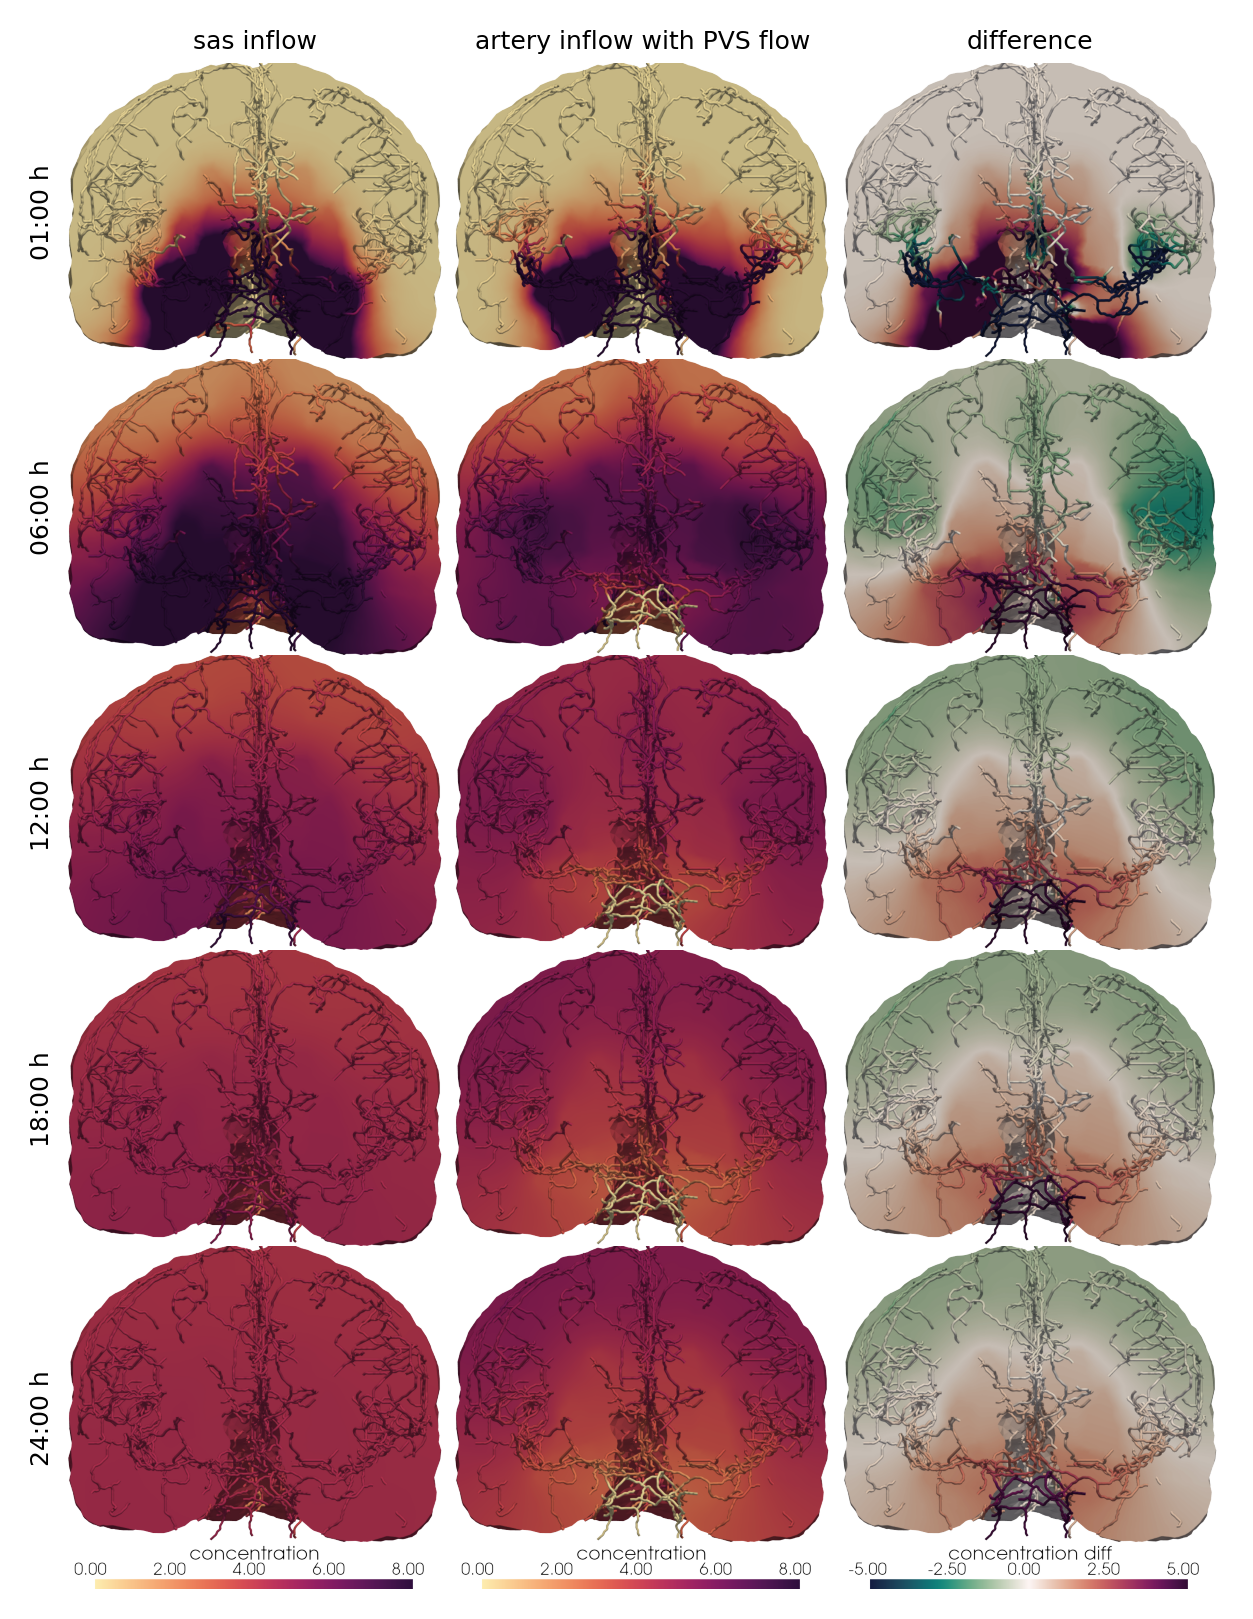
\includegraphics[width = 0.9 \textwidth]{modelB_modelC_overview.png}
    \caption{Tracer concentrations for a purely diffusive model with tracer inflow via the CSF-filled space (left) and a convective model with Tracer inflow via the arterial PVS (middle) and their difference (right) at 1, 6, 12, 18 and 24 hours after injection.}
    \label{fig:2}
\end{figure}
\subsection*{Effect of BBB}

Leakage to the blood, some sink/non-zero permeability for the PVS-blood (BBB) interface (Model N).

\begin{figure}
    \caption{}
    \label{fig:3}
\end{figure}

\subsection*{Effect of pia}
  
Effect of pia permeability (Model N-1)    

\begin{figure}
    \caption{}
    \label{fig:4}
\end{figure}

\begin{figure}
     \centering
     \begin{subfigure}[b]{0.33\textwidth}
         \centering
         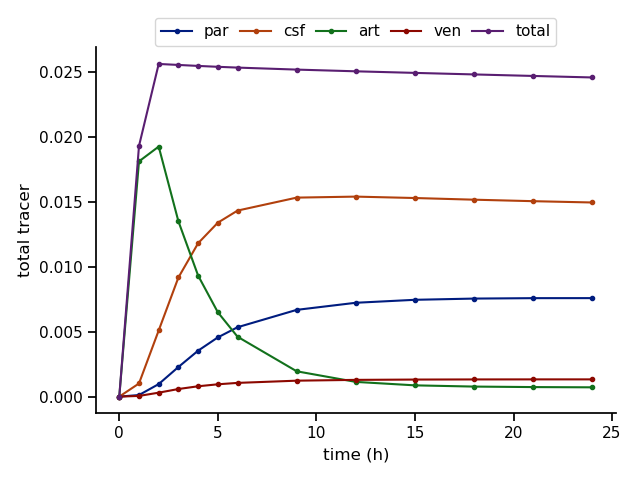
\includegraphics[width=\textwidth]{modelA_total_conc.png}
         \caption{arterial inflow, pure diffusion}
         \label{fig:y equals x}
     \end{subfigure}
     \hfill
     \begin{subfigure}[b]{0.33\textwidth}
         \centering
         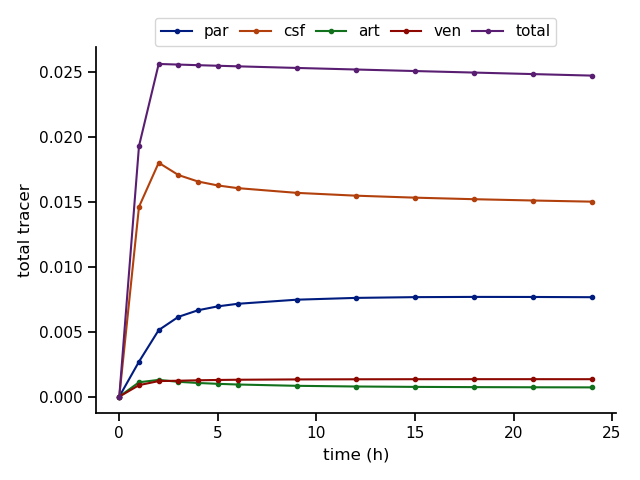
\includegraphics[width=\textwidth]{modelB_total_conc.png}
         \caption{SAS inflow, pure diffusion}
         \label{fig:three sin x}
     \end{subfigure}
     \hfill
     \begin{subfigure}[b]{0.33\textwidth}
         \centering
         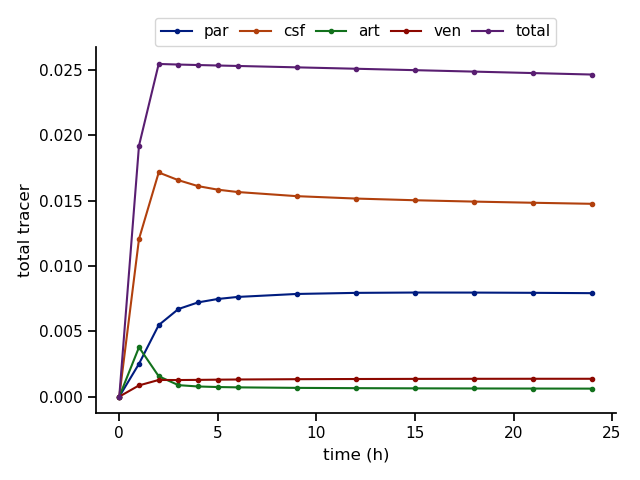
\includegraphics[width=\textwidth]{modelC_total_conc.png}
         \caption{arterial inflow, diffusion + PVS convection}
         \label{fig:five over x}
     \end{subfigure}
        \caption{Total tracer amount in parenchyma, CSF, arterial PVS and venous PVS}
        \label{fig:three graphs}
\end{figure}

\fi

\newpage
%%%%%%%%%%%%%%%%%%%%%%%%%%%%%%%%%%%%%%%%%%%%%%%%%%%%%%%%%%%%%%%%%%%%%%%%%%%%%%%%%%%%%
\section*{Methods}

%\mer{MER: I recommend writing each (sub)section of Methods as a nearly stand-alone paragraph. Let's see if we can avoid subsubsections/paragraphs. If you need to add more detail than you think is appropriate, put it in a Supplementary Methods section in the Appendix.} 

\subsection*{Brain parenchyma, SAS, and interface geometries}

\mer{MER: Suggestion @Rami: Would you have a go a refining this section? Keep it brief. Mention number of cells and max/min mesh size for both 3D and (peri)vasculature. I like including references to tools used as you have done. Refer to \Cref{fig:concept}. Include units when describing the geometry. Describe the radii provided. Describe the default assumption on the PVS size (probably we vary this in a model variation). Clearly illustrate the boundaries in the Figure, and refer to these in the text. Description should be such that it is easily to intuitively understand, but perhaps not reproduce immediately (that is why we will also share the code). }  


Hodneland et al~\cite{hodneland2019new} developed a method to image
the brains' microvasculature based on time-of-flight (ToF) and
quantitative susceptibility mapping (QSM) to identify arterial and
venous networks.  We derive a detailed tetrahedral mesh of the
parenchyma and the surrounding CSF-filled spaces alongside a network
representation of the vasculature from the anatomical data provided
therein. We merge the white and grey matter masks provided by
\cite{hodneland2019new} to extract the pial surface.
 


As no data on the CSF-filled spaces is available, we smooth and extend
the pial surface by about 5\,mm to obtain an approximation of the SAS
and include the inner fluid-filled cavities such as the ventricular
system.  Finally, we generate a tetrahedral mesh of both compartments
using the fTetWild meshing algorithm \cite{hu2020fast}.

The computational domain $\Omega$ is defined by the union of the SAS $\Omega_{\rm sas}$ and brain parenchyma $\Omega_{\rm brain}$. The thin pia membrane encloses the brain, and thus the pial surface (of the brain) defines the SAS-brain interface $\Gamma_{\rm pia}$.


Surface representations of the outer SAS boundary, pial membrane, and delimiters of other CSF-filled spaces such as the lateral ventricles, third and fourth ventricle, and aqueduct are extracted from MR-images of human subject(s), see e.g. the pipeline described by Hornkjøl et al.~\cite{hornkjol2022csf}. From these surface representations, we create volumetric meshes of the SAS and brain using SVMTK~\cite{mardal2022mathematical}. 

We mark the different regions of the boundary of $\Omega$, with
$\Gamma_{\mathrm{skull}}$ facing the dura and skull and
$\Gamma_{\mathrm{spine}}$ representing the lower interface towards the
spinal compartment (\Cref{fig:concept}). \mer{MER: I put this here, keep
  it here. How about the ventricles?}

\subsection*{Vascular and perivascular domains and networks}

We skeletonize the binary masks of the arteries and veins of the
Hodneland~\cite{hodneland2019new} data set using
Kiminaro~\cite{william_silversmith_2021_5539913}, to obtain the
centerline $\Gamma^i$ and radius $R_1^i$ of each detected vessel $i$,
and the vessel connections. The resulting vascular networks are
further smoothened using a spline interpolation technique, and
represented as graphs with nodes connected by edges. \mer{The nodes
  with the $m$ lowest z-coordinates are identified as the networks'
  root nodes, with $m = 3$ for the arterial network and $m = 50$ for
  the venous network. The arterial network has XXX nodes and YYY
  edges, while the venous network has XXX nodes and YYY edges in
  total.} We denote the domain defined by the connected centerlines by
$\Gamma$. The vascular domain is then represented as the union of
cylindrical vessels of radius $R_1^i$ surrounding the centerlines
$\Gamma^i$. Moreover, we consider the surrounding perivascular spaces
as the union of annular cylinders of inner radius $R_1^i$ and outer
radius $R_2^i = (1 + \alpha) R_1^i$ of width $R_2^i - R_1^i = \alpha
R_1^i$. Both the vasculature and perivasculature are thus defined
relative to a common network of vessel segments.

\begin{figure}
  \caption{\mer{MER: Concept figure illustrating the compartments and story line. (A) Concept sketch of the SAS, PVS and the brain; (B) Visualization of geometry domains (brain, sas and vasculature; think about colors and associations; please don't make blood blue and water red e.g.) ; (C) Zoom-in/detail on vasculature, which are which arteries (ACA, MCA, PCA, CoW)  and veins (XXX); (D) Zoom-in 2 on vascular position versus SAS and brain; (E) Zoom-in 3 on where PVS ends; (F) Illustration of boundaries? (G) Concept illustration of the mathematical model (diffusion, convection, exchange, boundaries).}}
\label{fig:concept}
\end{figure}

\subsection*{Multi-dimensional intracranial transport equations}

We model diffusion, convection and exchange of a solute in PVSs, in the surrounding SAS and in the brain parenchyma (Fig.~\ref{fig:concept}) via a comprehensive multi-dimensional transport model~\cite{masri2023modelling} over a timescale of minutes to hours. More specifically, we solve for a solute concentration $c$ in the 3D SAS and brain~\cite{sykova2008diffusion} $\Omega$, and an averaged solute concentration $\hat c$ in a 1D network of centerlines $\Lambda$ representing the PVS, such that the following equations hold
\begin{subequations}
\begin{alignat}{2}
  \partial_t (\phi c) - \nabla \cdot (D \nabla (\phi c) ) + \nabla \cdot (\bm u c ) + \xi (\overline{c} - \hat c ) \delta_\Gamma & = f && \quad \quad \mathrm{in} \quad \Omega, \\ 
  \partial_t (A \phi \hat c) - \partial_s(\hat D A \partial_s (\phi \hat c)) +\partial_s(A \hat u \hat c )  +  \xi P (\hat c - \overline{c})  &= A \hat f && \quad \quad \mathrm{in} \quad  \Lambda .
 \end{alignat}
\end{subequations}
Here $\phi$ is the fluid volume fraction (or porosity) of the brain (where $\phi \ll 1$), of the SAS (where $\phi = 1$) and of the PVS (where $0 \ll \phi \leq 1$); $D$ is the effective diffusion coefficient of the relevant solute in the respective media~\cite{sykova2008diffusion} which takes different values over the SAS, PVS, and tissue; $\bm u$ and $\hat u$ are convective velocity fields in $\Omega$ and $\Lambda$, respectively; $\xi$ is a transfer coefficient across the PVS-SAS interface; $P$ and $A$ are the perimeter and area of the PVS which can vary along the centerline network, respectively; and $f$ and $\hat{f}$ represents given sources of solute in $\Omega$ and $\Lambda$, respectively.  The (Dirac delta) term $\delta_\Gamma$ is a source term concentrated on the outer boundary of the PVS that models the solute exchange between the PVSs and their surroundings. Finally, the notation $\overline{c}$ denotes the lateral  average of the concentration over the outer perivascular boundary. Both $\Omega$ and $\Lambda$ are here fixed in time. We remark that this version of the model assumes that there is no interaction between the inner perivascular boundary and the blood vessel. 

%\noindent \mer{MER: @Rami: I've added the $\phi$'s in this subsection. Please review and add convective terms in $\Omega$ and $\Lambda$.} \rami{done, maybe I include a more precise variational formulation in the appendix ? }
\subsection*{Initial conditions}

We set the initial concentrations $c_0, \hat{c}_0$ in the three-dimensional domain $\Omega$ and network $\Lambda$ to be zero for all influx scenarios (Models A--\draft{X-1}). For modelling clearance (Model \draft{X}), we set $c_0 = 1, \hat{c}_0 = 0$.

\subsection*{Boundary conditions: extracranial efflux and perivascular parenchymal influx}

On the interface towards the dura and skull $\Gamma_{\mathrm{skull}}$, we consider a constant uptake (or efflux) rate, represented by the boundary condition $- D \nabla c \cdot \bm{n}  +   \bm u \cdot \bm n c  = \beta c $ (\Cref{fig:concept}) where $\beta$ represents a molecular outflow resistance. Here, we take $\beta = 10^{-4} \,\, \mathrm{mm}^2/\mathrm{s}$\cite{hornkjol2022csf}. On the interface towards the spinal compartment $\Gamma_{\mathrm{spine}}$, we prescribe a time-dependent solute influx rate by the condition $D \nabla c \cdot \bm{n}  -  \bm u \cdot \bm n  c = g_{\mathrm{influx}}(t) \geq 0$ representing the distribution of solute injected in the spinal compartment. Here, we set $g_\mathrm{influx}(t) = \max(0, \kappa (T_0 - t))$ where $\kappa  = $ and $T_0 = $ \rami{marius, double check in the code they are different than \cite{hornkjol2022csf}}. 

Similarly, on the associated perivascular network inlet nodes $\partial \Lambda_{\mathrm{in}}$ (\Cref{fig:concept}), we prescribe a compatible solute influx rate $\hat D A \partial_s (\phi \hat c) - A \hat u \hat c  = \hat g(t)$. \rami{The approach of setting $\hat g = 0$ and of setting the permeabitliy to be high (follows the arguments \cite{eide2024functional}) for the perivascular spaces that are near the spine, @Marius can you please add more details ? } For the "leaf" nodes of the perivascular network (representing the end of the surface perivascular network and start of perivascular spaces within the parenchyma), we also set a fixed transfer rate by setting $ D A \partial_s (\phi \hat c) - A \hat u \hat c  = g_{\mathrm{pvs-par}}$. \rami{I don't think we can have anything different than $g_{\mathrm{pvs-par}} = 0$ since we would also have to modify the 3D equation. The interaction b/w the pvs and the parenchyma is along the entire perivascular boundary as accounted for in the coupling terms}. 

\noindent \mer{MER: @Rami: I've edited this subsection. Maybe I've swapped the labeling of the network inlet and outlet nodes. Please review. We will probably discuss this a bit. A figure showing overview and details of the perivascular network will help in any case.}

%% For the network, the boundary nodes are split into $\partial \Lambda^{\mathrm{in}}$  and $\partial \Lambda^{\mathrm{out}}$ based on the specified orientation of the network (\color{blue} to be specified more precisely (with a figure?)\color{black}). We impose the following conditions. 
%% \begin{alignat}{2}
%% D A \partial_s \hat c &= 0, && \quad \mathrm{on} \,\, \partial \Lambda^ {\mathrm{in}}, \\ 
%% D A \partial_s  \hat c &= \hat g(t),  && \quad \mathrm{on} \,\, \partial \Lambda^{\mathrm{out}} .
%% \end{alignat}

\subsection*{Numerical approximation, implementation and verification}

\mer{MER: Who would like to draft a paragraph on our numerical approximation? @Miro? I recommend ``describing with words'' to reach relevant audiences. We need to demonstrate that our ``quantities are converged'', meaning we have a feel for how accurate our results are in practice (e.g.$\pm$ 1\%, 10\%, 100\%, 1000\%). Refer to the Supplementary table for a numerical verification table (quantities of interest versus mesh and time refinement for pure diffusion and one case with convection). Not on top of list of priorities, but not on bottom either.} 

\subsection*{Perivascular fluid flow}

\mer{MER: This we will probably have to condense. Move the detailed explanation to Supplementary Methods?}

We may consider non-zero convection in the SAS $u_{\rm sas} \not = 0$ e.g.~resulting from steady state CSF production as predicted by~\cite{hornkjol2022csf} in model variations, but may start with $u_{\rm sas} = 0$ as a baseline. In the perivascular network, we set an average axial velocity $u_{\rm pvs} = \langle u_{v, s} \rangle$ of $18.7$ $\mu$m/s as reported by Mestre et al.~\cite{mestre2018flow} in mouse perivascular spaces under normal physiological conditions. We may also consider a reduced perivascular velocity corresponding to hypertension in model variations.
\subsubsection*{Steady state PVS flow model} We solve 1D Darcy equations in the vessel network. The unknowns are the averaged PVS velocity, $u_{\rm pvs} = \langle u_{v,s} \rangle$, and the cross-section pressure $p_{\rm pvs} $ (assumed to be constant in each cross-section). The system is given by  \cite{daversin2022geometrically} 
\begin{alignat}{2}
A \,  u_{\rm pvs}   + \frac{\kappa}{\mu} \, A \, \partial_{s} p_{\rm pvs} & = 0, &&  \quad \rm in  \,\, \Lambda  \\ 
-\partial_s (A \, u_{\rm pvs}) & = f, && \quad \rm in  \,\, \Lambda .  
\end{alignat} 
In the above, $A$ is the area of the PVS, $\mu$ is the dynamic viscosity, and $\kappa$ is derived from the assumption of Poiseuille
flow in the annular cross-section of the PVS \cite{daversin2022geometrically,tithof2022network}: 
\begin{equation}
\kappa = \frac18 \left( R_2^2 + R_1^2 - \frac{1}{\ln(R_2/R_1)} (R_2^2- R_1^2) \right). 
\end{equation}
On bifurcations, conservation of fluxes is enforced weakly and continuity of the pressure is enforced strongly (in the choice of the finite element spaces). 

\subsubsection*{Case 1} We prescribe zero Dirichlet boundary conditions for the pressure, and vary $f$ \rami{include the reasoning behind having this $f$ as a source or sink term, and include the value that we opted for} to obtain a flow field with a similar magnitude to what is commonly reported in the literature.  

\subsection*{Case 2} We prescribe a Robin type boundary condition on the outlet nodes. In particular, we set 
\begin{equation}
A  u_{\rm pvs} =  - \frac{\kappa}{ \mu} A\, \partial_s p_{\rm pvs} = \alpha (p_{\rm pvs} - p_0), \quad  \rm on \,\,\, \partial \Lambda^{\rm out} 
\end{equation}
On $\partial \Lambda^{\rm in}$, we prescribe homogeneous Dirichlet data for the pressure (\rami{does this make sense?}). 
\rami{to be completed }

\subsection*{Cerebrospinal fluid flow in the subarachnoid space}

\draft{\lipsum[1]}

\subsection*{Fluid flow within the parenchyma}

We assume no significant convection in the brain $\Omega_{\rm brain}$, and set $u = u_{\rm brain} = 0$ there as a first approximation. 


\subsection*{Parameter values and model scenarios}
We use the diffusion coefficient $D_{\rm gad}$ of Gadubutrol in free water in the SAS and PVS, and effective diffusion coefficient of Gadubutrol $D_{\rm brain}$ -- accounting for the extracellular space (ECS) porosity $\phi$ and the ECS tortuosity $\lambda$ but ignoring anisotropy  -- in the brain parenchyma~\cite{hornkjol2022csf}. 
\begin{table}
  \begin{center}
    \begin{tabular}{ll|ccc}
      \toprule
      Parameter& Symbol & Value & Unit& Reference\\
      \midrule
         parenchyma app. diffusion&  $d_p$&  $1.2 \times 10^{-4}$& $\text{mm}^2/\text{s}$  & \cite{valnes2020apparent}\\
         CSF app. diffusion&  $d_{CSF}$&  $3.8 \times 10^{-4}$& $\text{mm}^2/\text{s}$ & \cite{valnes2020apparent}\\
         PVS diffusion&  $d_{PVS}$&  $3.8 \times 10^{-4}$& $\text{mm}^2/\text{s}$ & \cite{valnes2020apparent}\\
         extracellular space volume fraction& $\phi$& 0.2& - &\cite{nicholson1981ion} \\
         PVS-parenchyma permeability&  $\xi_{PVS,P}$& $5 \times 10^{2} - 6 \times 10^{3} $  & $\text{m}^{-1}$ & \cite{koch2023estimates} \\
         PVS-CSF permeability&  $\xi_{PVS,CSF}$& $\{0, \text{inf}\}$ & $\text{m}^{-1}$ & \\ 
         boundary concentration& $\hat{c}_D$& & &\\ \hline
         Extracranial efflux rate & $g_{\mathrm{efflux}}$  & 0 & mm$^2$/s \\
         Spinal solute influx rate & $g_{\mathrm{influx}}$ & $\max(0, a(T_0 - t))$  & mm$^2$/s
    \end{tabular}
  \end{center}
  \caption{Overview of physiological parameters and model variations. \mer{MER: This clearly needs some more work and probably would benefit from joint review. Should we look at it together, or does someone want to take the lead on collecting these?} \rami{apparent vs effective ? same thing ? need to use consistent names}}
  \label{tab:overview}
\end{table}


\begin{table}
\begin{center}
  \begin{tabular}{ll|llllll|ll}
    \toprule
    & Description & $R$ & $\xi_{\rm PVS-SAS}$, $\xi_{\rm PVS-PAR}$ & $\beta_{\rm efflux}$ & $D$ & $\hat{u}$ & $\mathbf{u}_{\rm SAS, brain}$ & $g_{\rm influx}$ & $c_0$ \\
    \midrule
    A & Baseline  & $R_2 = 2 R_1$ & $\xi$, $\tilde \xi$\cite{koch2023estimates} &  $10^{-4}$ mm$^2$/s\cite{hornkjol2022csf} & $D^{\rm gad}$\cite{sykova2008diffusion, valnes2020apparent}  & $\hat{u} = \hat{u}_{\rm prod}$ & $\mathbf{u}_{\rm SAS} = \mathbf{u}_{\rm prod}$, $\mathbf{u}_{\rm brain} = 0$ & $> 0$ & 0 \\
    B & PVS "sheaths" & $R_2 = 2 R_1$ & $0, 0.5 \xi, \xi, 2 \xi, 1000 \xi \approx \infty$, --\cite{koch2023estimates} & -- & --  &  --  & --  & -- & -- \\
    C & Larger PVS & $R_2 = N R_1$ & -- & -- & --  &  --  & -- & -- & -- \\
    D & PVS I & $R_2 = 2 R_1$ & $\xi$, -- & -- & --  &  $\hat{u} = \hat{u}_{\rm prod} + \uparrow$  & -- & -- & -- \\
    E & PVS II & $R_2 = 2 R_1$ & $\xi$, -- & -- & --  &  $\hat{u} = \hat{u}_{\rm prod} + \uparrow\uparrow$  & -- & -- & -- \\
    F & PVS III & $R_2 = 2 R_1$ & $\xi$, -- & -- & $10 D_{\rm PVS}$ &  $\hat{u} = \hat{u}_{\rm prod}$  & -- & -- & -- \\
    G & Glymphatics & $R_2 = 2 R_1$ & $\xi$, -- & -- & \cite{sykova2008diffusion, valnes2020apparent} &  $\hat{u} = \hat{u}_{\rm prod} + \uparrow$  & $\mathbf{u}_{\rm brain}$ > 0 & -- & -- \\
    H & Sleep &  &  & &  &  &  & & \\
    I & Pathology I &  &  & &  &  &  & & \\
    J & Pathology II &  &  & &  &  &  & & \\
    \midrule
    X & Clearance & $R_2 = 2 R_1$ & $50\%$, $\xi$ & -- & $D^{\rm gad, \tau, A\beta}$  &  $\hat{u} = \hat{u}_{\rm prod}$  & -- & $0$ & $1$ \\
    Y & (PVS) & $R_2 = 2 R_1$ & $50\%$, $\xi$ & -- & $D^{\rm gad, \tau, A\beta}$  &  $\hat{u} = \hat{u}_{\rm prod} + \uparrow$  & -- & -- & -- \\
    Z & (Glymphatic) & $R_2 = 2 R_1$ & $50\%$, $\xi$ & -- & $D^{\rm gad, \tau, A\beta}$  &  $\hat{u} = \hat{u}_{\rm prod} + \uparrow$  & $\mathbf{u}_{\rm brain}$ > 0 & -- & -- \\
    \bottomrule
    \end{tabular}
    \end{center}
\caption{Overview of models (-- denotes as immediately above). Model A represents a baseline scenario with semi-permeable barriers between the PVS and SAS ($\xi_{\rm PVS-SAS} \approx 50\%$, \mer{we try to estimate this value by a bit of trial-and-error from the observations of timings of PVS-SAS and SAS from~\cite{eide2024functional}})~\cite{bedussi2017paravascular} and astrocytic endfeet forming barriers within the parenchyma~\cite{koch2023estimates}. $R_1$ and $R_2$ denotes the inner and outer radius of the PVS, with PVS width comparable to vascular diameter ($R_2 - R_1 \approx 2 R_1$)\cite{mestre2018flow} as a baseline. The extracranial solute efflux permeability $\beta_{\rm efflux}$ is uniformly distributed over the outer SAS boundary with a reasonable rate as baseline\cite{hornkjol2022csf, eide2021clinical, ringstad2024glymphatic}. At baseline, the effective diffusion coefficients $D^{\rm x}_{\rm SAS} = D^{\rm x}_{\rm PVS}$ of the SAS and PVS represent the free diffusion coefficient of Gadubutrol (${\rm x} = {\rm gad}$) in CSF (water), and $D^{\rm x}_{\rm PAR}$ the effective diffusion coefficient of human cortical tissue, all at body temperature. At baseline, we consider net flow due to CSF-production in the SAS (and PVS): $\mathbf{u}_{\rm SAS} > 0$ (and $\hat{u} > 0$), but no additional effects from perivascular pulsatility nor bulk flow in the parenchyma $\mathbf{u}_{\rm brain} = 0$. Due to the timescale for human intracranial tracer transport (minutes to hours) compared to typical (cardiac, respiratory, slow vasomotion) human intracranial pulsatility (0.1 -- 1 Hz), we consider net (constant-in-time) flow fields only in subsequent model variations. Model B represents a PVS-SAS interface configuration with minimal or more permeable structural barriers~\cite{eide2024functional}, while Model C represents enlarged PVS. Models D, E, and F represent three perivascular pathway scenarios with more rapid flow in the PVS induced by vasomotion (PVS I)~\cite{gjerde2023directional} or a net fluid source in the PVS (1D Stokes flow)/net pressure difference between PVS inlets and outlets (PVS II), or with enhanced effective diffusion due to mixing (PVS III)~\cite{hornkjol2022csf, troyetsky2021dispersion, vinje2023human}, respectively. Model G attempts to represent a glymphatic--like convective flow within the parenchyma. \mer{Ideas could be:  (a) network induces arterial and venous sources in a Darcy porous media flow model (reflects the glymphatic hypothesis), (b) Croci-style \cite{croci2019uncertainty}, (c) \cite{vinje2023human}} Model H represents physiological alterations associated with sleep (lower CSF production, enhanced diffusion within the parenchyma, enhanced PVS pulsatility), while Models I--J represents variations associated with pathologies (e.g.~dementia, hypertension, angiopathies, CSF-disorders and/or others). Models X--Z represent version of the aforementioned scenarios but for studying metabolite clearance (instead of solute influx).}
  \label{tab:scenarios}
\end{table}


\mer{To be edited, just moved here:} We will consider different values for the SAS-PVS permeability $\xi$, including $\xi = 0$ (sealed PVS), $\xi \approx \infty$ (PVS continuous with SAS), as well as reasonable intermediate values. We will ignore PVS-blood exchange, and thus only model the perivascular concentration at the network level (in addition to the SAS/brain concentration in the surroundings).  

\subsection*{Quantities of interest}

\begin{itemize}
    \item Snapshots (e.g. coronal plane) of concentration at relevant times (15 min, 30 min, 1h, 2h, ...) 
    \item Total amount of tracer in the PVS, SAS and parenchyma
     \item Time to reach a threshold (e.g. 30\%) in different "places"
\end{itemize}


%%%%%%%%%%%%%%%%%%%%%%%%%%%%%%%%%%%%%%%%%%%%%%%%%%%%%%%%%%%%%%%%%%%%%%%%%%%%%%%%%%%%%
\section*{Discussion}

\subsection*{Limitations}

\begin{itemize}
\item
  Pulsating brain. Natural to consider in follow-up work.
\item
  PVS-blood exchange and BBB leakage. Natural to consider in model variation here, or follow-up work.
\item
  Accounting for brain diffusive anisotropy. Little effect expected. Maybe something to consider in small follow-up work.
\item
  Permeability and stiffness of the pial membrane
\end{itemize}

\bibliography{references}

\newpage
\section*{Acknowledgments (not compulsory)}

Acknowledgments should be brief, and should not include thanks to anonymous referees and editors, or effusive comments. Grant or contribution numbers may be acknowledged.

\section*{Author contributions statement}

Must include all authors, identified by initials, for example:
A.A. conceived the experiment(s),  A.A. and B.A. conducted the experiment(s), C.A. and D.A. analysed the results.  All authors reviewed the manuscript. 

\section*{Additional information}

To include, in this order: \textbf{Accession codes} (where applicable); \textbf{Competing interests} (mandatory statement). 

The corresponding author is responsible for submitting a \href{http://www.nature.com/srep/policies/index.html#competing}{competing interests statement} on behalf of all authors of the paper. This statement must be included in the submitted article file.


\newpage
\appendix

\section{Supplementary methods}

\subsection{Numerical verification}

\mer{MER: Good place for numerical verification text and table. And more description of numerics if you would like.}


\newpage
\section{Notes}

Various notes associated with \cite{eide2024functional}:
\begin{itemize}
  \item
    Can observations of tracer indicate compartmentalization without
    the existence of physical barriers but in the presence of
    e.g.~substantial flow? We made observations in this direction in
    \cite{vinje2021brain}, relating to the then-active
    shape-of-perivascular-spaces discussion. We can address this by
    trying to quantify and evaluate the permeability of the PVS-SAS
    interface - comparing model predictions with the timings and
    patterns presented by \cite{eide2024functional}.
  \item
    Do the tracer primarily move from the PVS into the SAS or along
    (more slowly) along the SAS? This is left as an open question by
    \cite{eide2024functional} (page 3)
  \item
    How do altered ICP affect transport? Note that PVSAS transport is
    impaired (delayed) with increasing mean wave amplitude in the ICP
    signal and for iNPH patients (with enlarged PVSAS spaces).
  \item
    Very useful reference for PVS sizes (10--20 mm$^2$ in reference
    patients, 15-70 mm$^2$ in iNPH), and average propagation speeds.
\end{itemize}

\end{document}
